\paragraph{Description of the datasets}
A suitable \ac{BCI} corpus was selected based on a preliminary screening, based
on its large interdependence of classification errors close in time.
%
This corpus contains \ac{EEG} signals for 12 subjects, recorded during 30
minutes of natural game play, synchronized with annotations of key presses. The
game was designed to evoke changes in the mental state by periodically ignoring
15\% of the keyboard input. Please refer to Chapter~\ref{chap:loc} for
experimental details. Due to the unconstrained nature of this game, the key
strokes follow each other rather quickly. While this dataset satisfies the
non-\ac{IID} assumption of the \ac{dSVM}, the disadvantage of this dataset is
that the short trials might make the task-related signals undetectable, as the
recommended \ac{ITI} for the motor related \ac{ERD} is at least 10~sec
\cite{pfurtscheller1999eem}. 

% Recording
A BioSemi ActiveTwo \ac{EEG} system was used to record 32 channels of \ac{EEG}
and physiological signals at a sampling rate of 512~Hz. The 32 Ag/AgCl active
electrodes were placed at locations of the Extended International 10-20 system.
To measure the influence of ocular and muscle artifacts, \acs{EOG} (horizontal
and vertical pairs) and two pairs of \acs{EMG} signals over the left and right
flexor digitorum profundus (the muscles used to press with the index finger)
were recorded.

% Preprocessing
\begin{sloppypar}
For this chapter, the recordings were preprocessed as follows: first the
recording was downsampled to 128 Hz to speed up processing. After downsampling,
the data was high-pass filtered using a 4th-order Butterworth filter to remove
frequencies below 0.2 Hz, and notch-filtered using a 4th-order Butterworth
filter from 49--51 Hz to remove power line noise. The \ac{EEG} was then
corrected for eye movements using a regression  based subtraction method
\cite{schloegl2007fac}.
\end{sloppypar}

\begin{figure}
  \center
  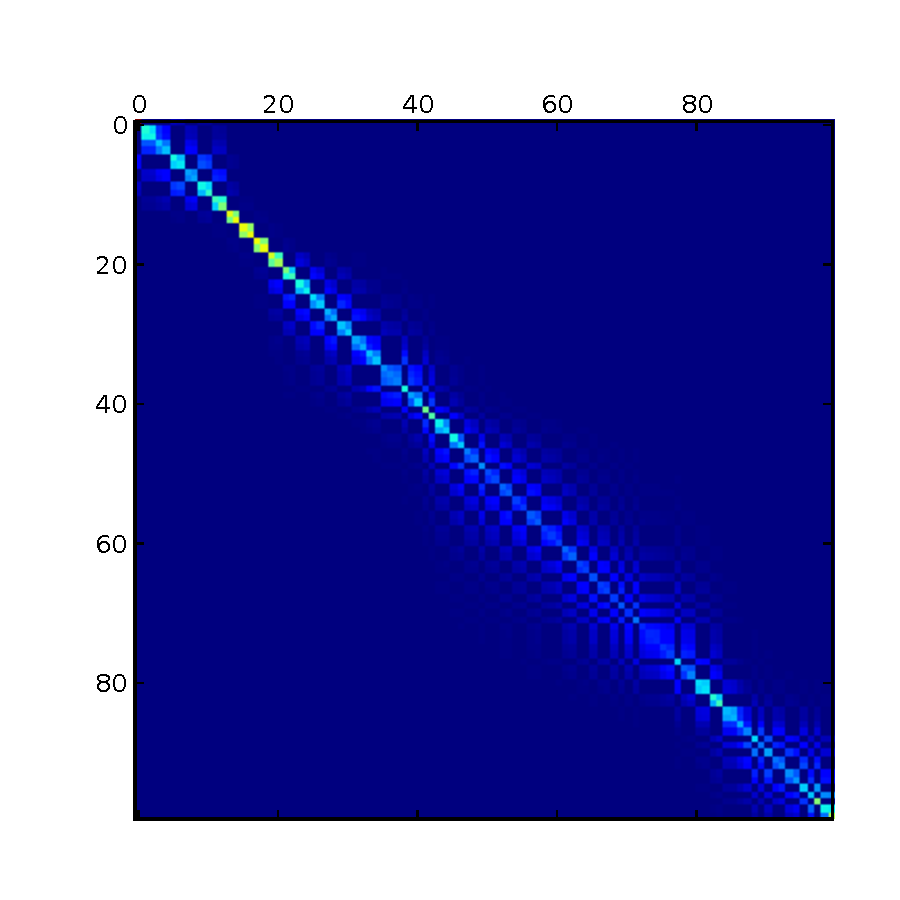
\includegraphics[width=.5\textwidth]{s0_D}
  \caption{An color-coded example dispersion matrix $D$ for the first 100
  trials of subject S0. The used dependence function is a Laplace distribution
  with width $b=2$ for trials of the same class. The green diagonal entries
  around trial 20 indicate independent trials, while the pattern around trial 60
  indicates a closely packed group of trials that are interdependent.}
  \label{fig:ex_D}
\end{figure}

% Feature extraction
\paragraph{Feature extraction}
After preprocessing, the signals were filtered with a 6th-order Butterworth
bandpass filter with a passband of 8--30~Hz, windows of 1~sec centered on the
moment the key-press was registered were extracted, and the Ledoit-Wolf
covariance estimator \cite{ledoit2004wce} was used to estimate the
channel-covariance in the trial window. Finally, a symmetrical whitening
transform $P = \Sigma^{-\frac{1}{2}}$ based on the mean channel covariance
matrix $\Sigma$ was calculated on the training set, and applied to all trials.
The resulting $32\times32$ features were vectorized and used for
classification. This pipeline is conceptually similar to the popular \ac{CSP}
based \cite{koles1991qet, ramoser2000osf} classification of \ac{ERD} related to
movement imagery, but it delegates learning of the spatial filters to the
classifier. 

\paragraph{Performance evaluation}
For \ac{BCI} data it is expected that the \ac{IID} data assumption does not
hold, as there are non-stationary perturbations in the data. This complicates
the evaluation procedure as one cannot simply use cross-validation when the
trials (instances) are inter-dependent. We opted for a simulation
approach, in which we used the first 800 trials for training, used the
performance on the following 400 trials for model selection, and used the
remaining $\approx 800$ trials as the test set. Nevertheless, non-stationary
perturbations could be present in the validation and test set, and could skew
the results, as the performance is measured based on the \ac{IID} assumption.
To improve the robustness of the performance measure, both the validation and
test sets were split into five continuous parts, and the median of the
performance on each part was used.
%
As a measure of performance we chose to use the \ac{ITR} based on \ac{MI}
between the predictions and the true class labels, which is an
information-theoretic measure of the communication speed through an unreliable
communication channel (the \ac{BCI}). The advantage of \ac{ITR} over, for
example, accuracy is that it takes both the quality of the prediction and the
speed of communication into account.

\begin{table}
  \caption{The \protect\ac{ITR} for the \protect\ac{SVM} and \protect\ac{dSVM}
  classifiers. \protect\acp{ITR} below 1 bit/min have been removed for clarity.} 
  \label{tab:dsvm_itr}
  \begin{center}

  \begin{tabular}{c D{.}{.}{3} D{.}{.}{3} D{.}{.}{2}}
    \toprule
    Subject & 
      \multicolumn{1}{c}{\ac{SVM} bits/min} & 
      \multicolumn{1}{c}{\ac{dSVM} bits/min} & 
      \multicolumn{1}{c}{b-param}\\
    \midrule
    S0 & 5.26 & 6.38 & 1.3\\
    S1 & - & - & 0.01\\
    S2 & - & - & 8.9\\
    S3 & - & - & 0.48\\
    S4 & - & 1.02 & 0.11\\
    S5 & 11.9 & 11.2 & 0.11\\
    S6 & - & - & 5.5\\
    S7 & - & - & 38\\
    S8 & - & - & 8.9\\
    S9 & 13.8 & 18.0 & 0.3\\
    S10 & 2.58 & 5.1 & 1.3\\
    S11 & -& - & 2.1\\
    \bottomrule
  \end{tabular}
  \end{center}
\end{table}

\begin{figure}
  \center
  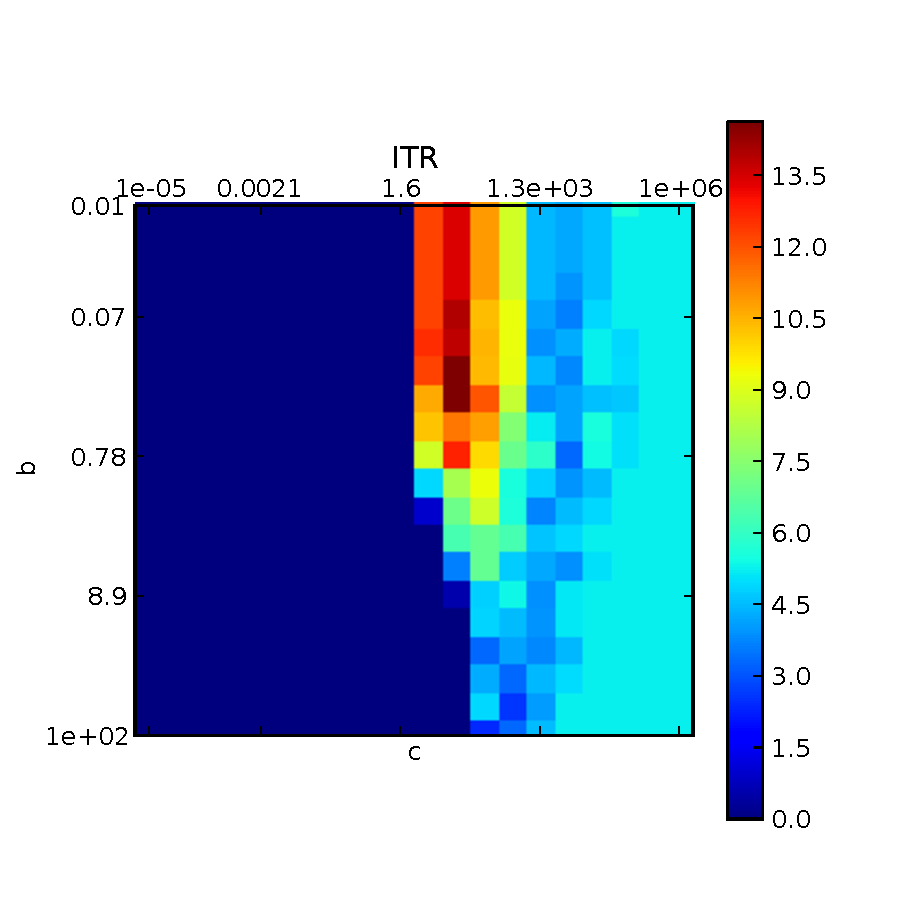
\includegraphics[width=.5\textwidth]{s9_itr_grid}
  \caption{The \protect\ac{ITR} on the test set of S9 for different
  combinations of the cost parameter $c$ and dispersion parameter $b$. The top
  row has such a small $b$ that the \protect\ac{dSVM} degenerates in the
  traditional \protect\ac{SVM}. The optimal spread appears to be $b=0.3$, which
  indicates that modeling the inter-dependency of trials is beneficial for this
  subject.}
  \label{fig:s9_itrgrid}
\end{figure}

\paragraph{Results} 
On the training and validation set, we performed a grid-search with the
soft-margin \acp{SVM} and the \acp{dSVM} with different cost parameters $c$,
and different width parameters $b$ in \eqref{eq:dfunc} for the \ac{dSVM} (see
Figure~\ref{fig:ex_D} for an example of the resulting $D$) with a linear,
inhomogeneous kernel. The offset parameter $\mu$ in \eqref{eq:dfunc} was set to
zero.
%
The performance of the selected \ac{SVM} and \ac{dSVM} classifiers are
presented in Table~\ref{tab:dsvm_itr}. Unfortunately, for a number of subjects
no well-performing classifier could be trained with either classifier. For the
subjects for which a classifier could be trained, the \ac{dSVM} seems to
outperform the standard soft-margin \ac{SVM}, with S5 being the only (minor)
exception. The best subject displays a dramatic improvement in performance,
from 13.8 to 18.0 bits per minute (see Figure~\ref{fig:s9_itrgrid}).
